\chapter{Project Management \& Financing}

\section{Work Breakdown Structure (WBS)}
To ensure systematic development and timely delivery of the Car Sales Management System, I developed a comprehensive Work Breakdown Structure (WBS) prior to implementation. I decomposed the project into ten Level-1 deliverable packages: Project Setup \& Configuration, Database Design \& Data Modeling, Internal ERP/CRM (\texttt{car\_sales}), Customer E-Commerce (\texttt{ecommerce}), Authentication \& Authorization, API Development, Analytics \& Reporting, Messaging \& Notifications, Frontend UI Templates, and Testing \& Deployment. I further broke down each Level-1 package into concrete Level-2 work packages that map directly to the models, views, and API endpoints I implemented in the codebase, ranging from environment setup and schema design (1.1--2.8), through entity CRUD, catalog, and checkout logic (3.1--4.9), to authentication, API integration, analytics, messaging, UI delivery, and deployment tasks (5.1--10.5). Structuring the WBS this way allowed me to track granular progress against each module and directly informed both the dependency chain and the Gantt chart schedule.

\begin{figure}[H]
\centering
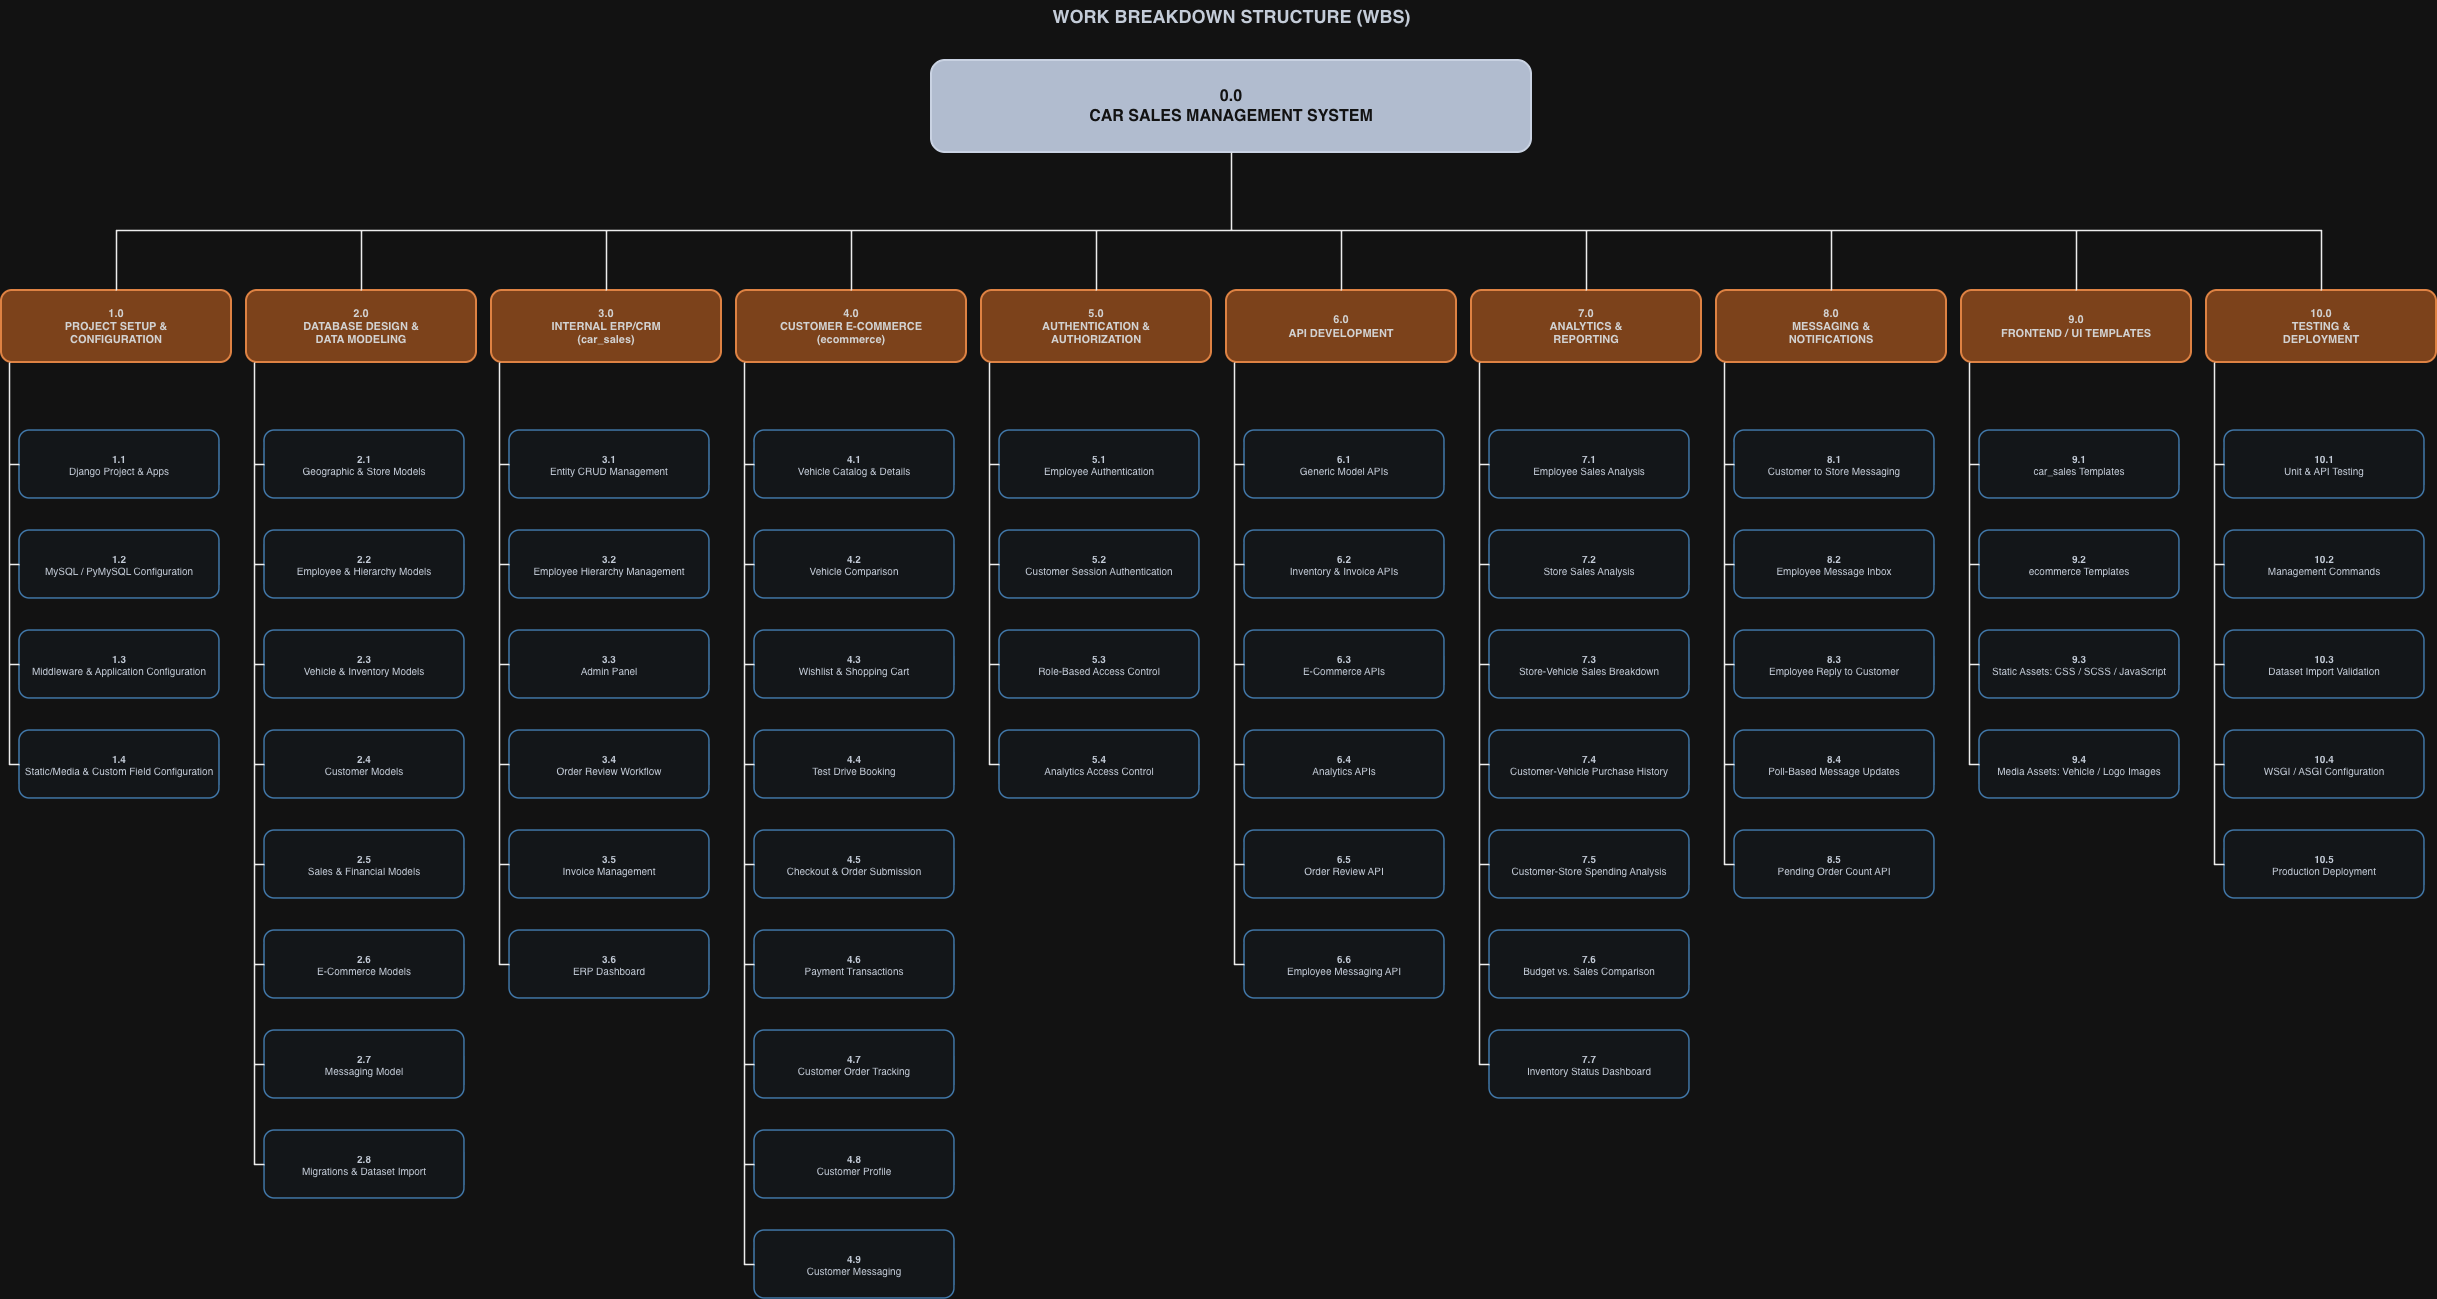
\includegraphics[width=\textwidth]{images/wbs.png}
\caption{Work Breakdown Structure (WBS) - Car Sales Management System}
\label{fig:wbs_diagram}
\end{figure}

\section{Process/Activity-Wise Time Distribution}

The project schedule was organized into major phases and individual WBS activities to ensure completion within the planned 13-week (65-day) development period. Rather than sequencing activities arbitrarily, I derived the schedule from technical dependencies between components: an activity could only begin once every prerequisite task (whether a model, an endpoint, or a view) was completed. For instance, API endpoints (Phase 6.0) could not be built before their underlying models (Phase 2.0) and authentication layer (Phase 5.0) existed, and frontend templates (Phase 9.0) required finalized APIs and views (Phases 3.0, 4.0, and 6.0). Table~\ref{tab:time-distribution} presents the estimated working days, start and end days, and dependencies assigned to each of the 60 Level-2 activities across all ten WBS phases, using a Day-1-start convention consistent with the Gantt chart in Figure~\ref{fig:gantt_chart}. The Dependencies column was subsequently used as the input network for the Critical Path Method analysis discussed below.

\pagebreak
\renewcommand{\arraystretch}{1.25}
\setlength{\tabcolsep}{5pt}
\scriptsize

\begin{longtable}{@{}p{3cm}p{5.5cm}rrrp{1.8cm}@{}}
\caption{Scheduling assumption: The project runs for 13 weeks.}
\label{tab:time-distribution}\\

\toprule
\textbf{Phase} & \textbf{Activity} &
\textbf{Days} & \textbf{Start} & \textbf{End} & \textbf{Dependencies} \\
\midrule
\endfirsthead

\toprule
\textbf{Phase} & \textbf{Activity} &
\textbf{Days} & \textbf{Start} & \textbf{End} & \textbf{Dependencies} \\
\midrule
\endhead

\midrule
\multicolumn{6}{r}{\textit{Continued on next page}} \\
\endfoot

\bottomrule
\endlastfoot

1.0 Project Setup \& Configuration
& 1.1 Django Project \& Apps & 1 & 1 & 1 & --- \\
1.0 Project Setup \& Configuration
& 1.2 MySQL / PyMySQL Configuration & 1 & 2 & 2 & 1.1 \\
1.0 Project Setup \& Configuration
& 1.3 Middleware \& Application Configuration & 1 & 3 & 3 & 1.2 \\
1.0 Project Setup \& Configuration
& 1.4 Static/Media \& Custom Field Configuration & 1 & 4 & 4 & 1.3 \\

2.0 Database Design \& Data Modeling
& 2.1 Geographic \& Store Models & 1 & 5 & 5 & 1.4 \\
2.0 Database Design \& Data Modeling
& 2.2 Employee \& Hierarchy Models & 1 & 6 & 6 & 2.1 \\
2.0 Database Design \& Data Modeling
& 2.3 Vehicle \& Inventory Models & 2 & 7 & 8 & 2.1 \\
2.0 Database Design \& Data Modeling
& 2.4 Customer Models & 1 & 9 & 9 & 2.1 \\
2.0 Database Design \& Data Modeling
& 2.5 Sales \& Financial Models & 1 & 10 & 10 & 2.2, 2.3, 2.4 \\
2.0 Database Design \& Data Modeling
& 2.6 E-Commerce Models & 1 & 11 & 11 & 2.3, 2.4 \\
2.0 Database Design \& Data Modeling
& 2.7 Messaging Model & 1 & 12 & 12 & 2.2, 2.4 \\
2.0 Database Design \& Data Modeling
& 2.8 Migrations \& Dataset Import & 1 & 13 & 13 & 2.1--2.7 \\

3.0 Internal ERP/CRM System
& 3.1 Entity CRUD Management & 1 & 14 & 14 & 2.8 \\
3.0 Internal ERP/CRM System
& 3.2 Employee Hierarchy Management & 1 & 15 & 15 & 3.1 \\
3.0 Internal ERP/CRM System
& 3.3 Admin Panel & 1 & 16 & 16 & 3.1 \\
3.0 Internal ERP/CRM System
& 3.4 Order Review Workflow & 1 & 17 & 17 & 2.5, 3.1 \\
3.0 Internal ERP/CRM System
& 3.5 Invoice Management & 1 & 18 & 18 & 3.4 \\
3.0 Internal ERP/CRM System
& 3.6 ERP Dashboard & 2 & 19 & 20 & 3.2, 3.3, 3.5 \\

4.0 Customer E-Commerce System
& 4.1 Vehicle Catalog \& Details & 1 & 21 & 21 & 2.8 \\
4.0 Customer E-Commerce System
& 4.2 Vehicle Comparison & 1 & 22 & 22 & 4.1 \\
4.0 Customer E-Commerce System
& 4.3 Wishlist \& Shopping Cart & 1 & 23 & 23 & 4.1 \\
4.0 Customer E-Commerce System
& 4.4 Test Drive Booking & 1 & 24 & 24 & 4.1 \\
4.0 Customer E-Commerce System
& 4.5 Checkout \& Order Submission & 2 & 25 & 26 & 4.3 \\
4.0 Customer E-Commerce System
& 4.6 Payment Transactions & 1 & 27 & 27 & 4.5 \\
4.0 Customer E-Commerce System
& 4.7 Customer Order Tracking & 1 & 28 & 28 & 4.6 \\
4.0 Customer E-Commerce System
& 4.8 Customer Profile & 1 & 29 & 29 & 2.4 \\
4.0 Customer E-Commerce System
& 4.9 Customer Messaging & 1 & 30 & 30 & 2.7, 4.8 \\

5.0 Authentication \& Authorization
& 5.1 Employee Authentication & 1 & 31 & 31 & 2.2 \\
5.0 Authentication \& Authorization
& 5.2 Customer Session Authentication & 1 & 32 & 32 & 2.4 \\
5.0 Authentication \& Authorization
& 5.3 Role-Based Access Control & 1 & 33 & 33 & 5.1 \\
5.0 Authentication \& Authorization
& 5.4 Analytics Access Control & 1 & 34 & 34 & 5.3 \\

6.0 API Development
& 6.1 Generic Model APIs & 1 & 35 & 35 & 5.3 \\
6.0 API Development
& 6.2 Inventory \& Invoice APIs & 1 & 36 & 36 & 3.5, 5.3 \\
6.0 API Development
& 6.3 E-Commerce APIs & 1 & 37 & 37 & 4.5, 5.2 \\
6.0 API Development
& 6.4 Analytics APIs & 1 & 38 & 38 & 2.5, 5.4 \\
6.0 API Development
& 6.5 Order Review API & 1 & 39 & 39 & 3.4, 5.3 \\
6.0 API Development
& 6.6 Employee Messaging API & 1 & 40 & 40 & 2.7, 5.1 \\

7.0 Analytics \& Reporting
& 7.1 Employee Sales Analysis & 1 & 41 & 41 & 6.4 \\
7.0 Analytics \& Reporting
& 7.2 Store Sales Analysis & 1 & 42 & 42 & 6.4 \\
7.0 Analytics \& Reporting
& 7.3 Store-Vehicle Sales Breakdown & 1 & 43 & 43 & 6.4 \\
7.0 Analytics \& Reporting
& 7.4 Customer-Vehicle Purchase History & 1 & 44 & 44 & 6.4 \\
7.0 Analytics \& Reporting
& 7.5 Customer-Store Spending Analysis & 1 & 45 & 45 & 6.4 \\
7.0 Analytics \& Reporting
& 7.6 Budget vs.\ Sales Comparison & 1 & 46 & 46 & 6.4 \\
7.0 Analytics \& Reporting
& 7.7 Inventory Status Dashboard & 2 & 47 & 48 & 6.2, 6.4 \\

8.0 Messaging \& Notifications
& 8.1 Customer-to-Store Messaging & 1 & 49 & 49 & 4.9, 6.6 \\
8.0 Messaging \& Notifications
& 8.2 Employee Message Inbox & 1 & 50 & 50 & 6.6 \\
8.0 Messaging \& Notifications
& 8.3 Employee Reply to Customer & 1 & 51 & 51 & 8.2 \\
8.0 Messaging \& Notifications
& 8.4 Poll-Based Message Updates & 1 & 52 & 52 & 8.1, 8.3 \\
8.0 Messaging \& Notifications
& 8.5 Pending Order Count API & 1 & 53 & 53 & 6.2 \\

9.0 Frontend / UI Templates
& 9.1 \texttt{car\_sales} Templates & 2 & 54 & 55 & 3.6, 6.1 \\
9.0 Frontend / UI Templates
& 9.2 \texttt{ecommerce} Templates & 2 & 56 & 57 & 4.7, 6.3 \\
9.0 Frontend / UI Templates
& 9.3 Static Assets: CSS / SCSS / JavaScript & 2 & 58 & 59 & 9.1, 9.2 \\
9.0 Frontend / UI Templates
& 9.4 Media Assets: Vehicle / Logo Images & 1 & 60 & 60 & 9.3 \\

10.0 Testing \& Deployment
& 10.1 Unit \& API Testing & 1 & 61 & 61 & 6.1--6.6, 9.4 \\
10.0 Testing \& Deployment
& 10.2 Management Commands & 1 & 62 & 62 & 2.8 \\
10.0 Testing \& Deployment
& 10.3 Dataset Import Validation & 1 & 63 & 63 & 2.8, 10.2 \\
10.0 Testing \& Deployment
& 10.4 WSGI / ASGI Configuration & 1 & 64 & 64 & 10.1 \\
10.0 Testing \& Deployment
& 10.5 Production Deployment & 1 & 65 & 65 & 10.1, 10.3, 10.4 \\

\midrule
\textbf{Total}
& \textbf{Total Estimated Development Time}
& \textbf{65} & \textbf{1} & \textbf{65} & \\

\end{longtable}

\normalsize

\section{Gantt Chart}
To translate the Work Breakdown Structure into an actionable execution timeline, I developed a 13-week (65-day) project schedule using a Gantt chart, sequencing the ten major development phases from initial setup through final deployment. I structured the timeline so that foundational work precedes dependent modules: Project Setup \& Configuration (Days 1--4) and Database Design \& Data Modeling (Days 5--13) were scheduled first, since every subsequent phase relies on a stable schema and development environment. I then allocated Days 14--20 to the Internal ERP/CRM System and Days 21--30 to the Customer E-Commerce System (\texttt{ecommerce}), running these back-to-back rather than in parallel to reflect my solo-developer capacity and to allow lessons from the ERP build to inform the e-commerce implementation.

I placed Authentication \& Authorization (Days 31--34) after both core systems were functionally scaffolded, since securing endpoints meaningfully requires the routes and models to already exist. API Development (Days 35--40) follows immediately after, exposing the now-authenticated ERP and e-commerce functionality to external consumers. I scheduled Analytics \& Reporting (Days 41--48) and Messaging \& Notifications (Days 49--53) as largely sequential, lower-dependency phases that layer on top of the completed core, followed by Frontend/UI Templates (Days 54--60) once the underlying APIs were stable enough to build interfaces against. I reserved the final phase, Testing \& Deployment (Days 61--65), as a dedicated closeout window for integration testing, bug fixes, and release preparation across the entire system.

Overall, I designed the schedule to be front-loaded on architecture and data modeling, since I judged that errors made early in the schema would be the most expensive to fix later, and back-loaded on validation, giving the project a full week of buffer for testing before delivery.

\begin{figure}[H]
\centering
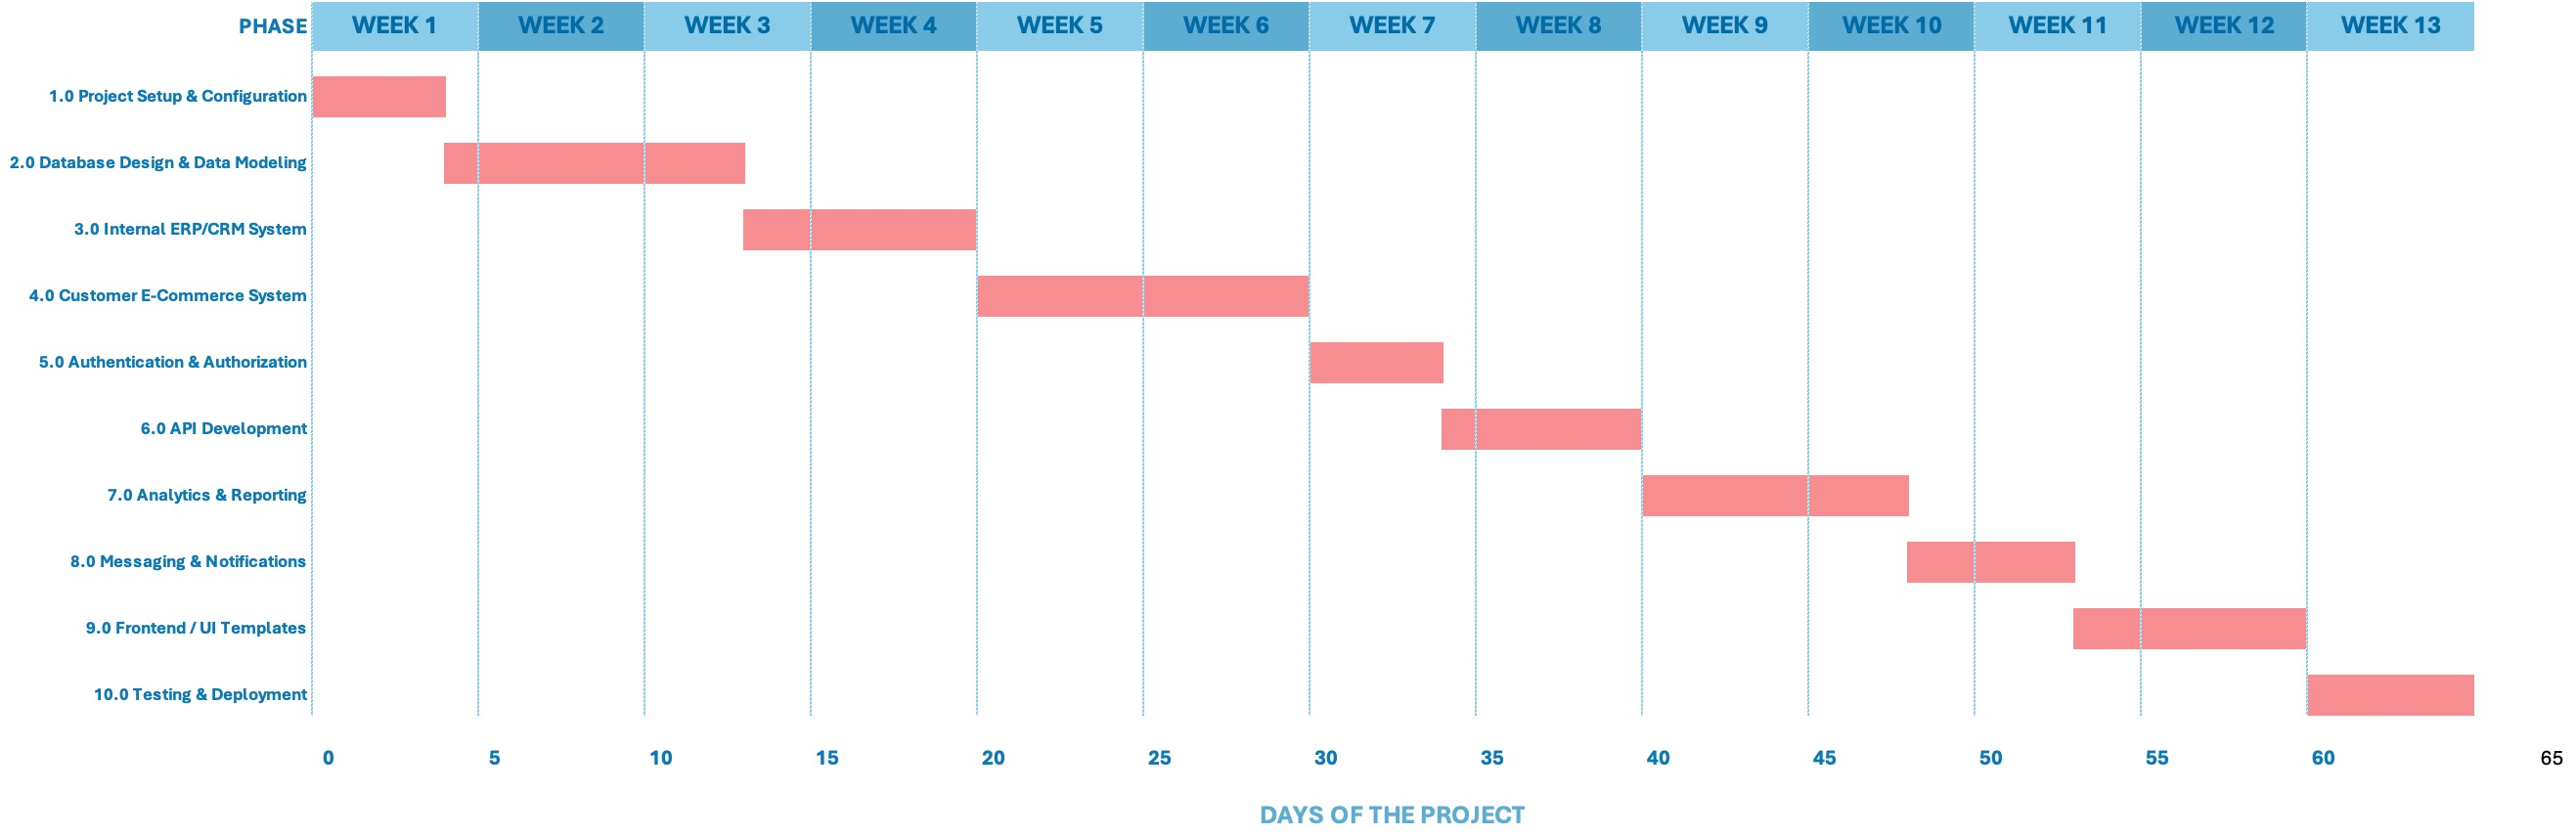
\includegraphics[width=\textwidth]{images/Gantt_Chart.jpg}
\caption{Project Execution Timeline (Gantt Chart) - Car Sales Management System}
\label{fig:gantt_chart}
\end{figure}

\section{Process/Activity wise Resource Allocation}

Since I completed this project as a solo developer, "resource allocation" in this context does not refer to distributing tasks across multiple team members, but to the distribution of my own effort across the distinct functional roles a real development team would normally divide among specialists: Database Design, Backend/API Development, Frontend Development, Quality Assurance (QA) \& Testing, and DevOps/Environment Configuration. I estimated the proportion of each phase's effort that fell into each role based on the nature of the work performed, for example, Database Design \& Data Modeling (Phase 2.0) was almost entirely Database Designer effort, while Frontend/UI Templates (Phase 9.0) was predominantly Frontend Developer effort with a smaller QA component for cross-browser and layout verification. Figure~\ref{fig:resource_allocation} visualizes this role-wise effort distribution (in person-days) across all ten WBS phases, and Table~\ref{tab:resource-summary} summarizes the total person-days and percentage share contributed by each role over the full 65-day schedule.

\begin{figure}[H]
\centering
\resizebox{\textwidth}{!}{%
\begin{tikzpicture}
\begin{axis}[
    xbar,
    width=15cm,
    height=13cm,
    bar width=22pt,
    xlabel={Days},
    xlabel style={font=\bfseries\color{ganttblue}},
    symbolic y coords={DevOps,QA/Tester,Frontend Developer,Backend/API Developer,Database Designer},
    ytick=data,
    y tick label style={font=\bfseries\small, color=ganttblue, align=right},
    xtick={0,5,10,15,20,25,30},
    xmin=0, xmax=32,
    enlarge y limits=0.15,
    axis line style={draw=none},
    tick style={draw=none},
    xmajorgrids=true,
    grid style={dashed, gray!30},
    nodes near coords,
    nodes near coords align={horizontal},
    nodes near coords style={font=\bfseries\small, color=ganttblue, xshift=4pt},
    every node near coord/.append style={anchor=west},
]
\addplot+[fill=ganttcoral, draw=none, fill opacity=0.85] coordinates {
    (4.80,DevOps)
    (7.45,Frontend Developer)
    (10.75,Database Designer)
    (13.00,QA/Tester)
    (29.00,Backend/API Developer)
};
\end{axis}
\end{tikzpicture}%
}
\caption{Process/Activity-Wise Resource (Role) Allocation - Car Sales Management System}
\label{fig:resource_allocation}
\end{figure}

\begin{table}[H]
\centering
\renewcommand{\arraystretch}{1.5}
\resizebox{0.75\textwidth}{!}{%
\begin{tabular}{@{}lrr@{}}
\toprule
\textbf{Resource Role} & \textbf{Days} & \textbf{\% of Total Effort} \\
\midrule
Database Designer                & 10.75 & 16.5\% \\
Backend / API Developer         & 29.00 & 44.6\% \\
Frontend Developer               & 7.45  & 11.5\% \\
QA / Tester                     & 13.00 & 20.0\% \\
DevOps / Environment Configuration & 4.80 & 7.4\% \\
\midrule
\textbf{Total}                   & \textbf{65.00} & \textbf{100\%} \\
\bottomrule
\end{tabular}%
}
\caption{Total Resource (Role) Allocation Summary}
\label{tab:resource-summary}
\end{table}

As the table shows, I allocated the largest share of effort, roughly 45\%, to Backend/API Development, which is consistent with the fact that Phases 3.0 through 8.0 (ERP, E-Commerce, Authentication, API, Analytics, and Messaging) are all primarily server-side work. QA/Testing effort (20\%) was distributed across nearly every phase rather than concentrated only in Phase 10.0, reflecting my practice of writing and running tests incrementally alongside each module rather than deferring all validation to the end. Database Design (16.5\%) and Frontend Development (11.5\%) were more front-loaded and back-loaded respectively, occurring predominantly in Phase 2.0 and Phase 9.0, while DevOps effort (7.4\%) was concentrated at the very beginning (environment setup) and very end (production deployment) of the timeline.